\documentclass[11pt,border=5pt]{standalone}
\usepackage[T1]{fontenc}
\usepackage{lmodern}
\IfFileExists{Jost.sty}{\usepackage{Jost}}{}
\usepackage{pgfplots}
\usepgfplotslibrary{fillbetween}
\pgfplotsset{compat=1.18}
\usepackage{xcolor}

\definecolor{teal}{HTML}{004D40}
\definecolor{coral}{HTML}{FF655D}
\definecolor{yellow}{HTML}{F1DB4B}
\definecolor{lightcoral}{HTML}{FF655D}
\definecolor{lightgray}{HTML}{D0D0D0}

\begin{document}
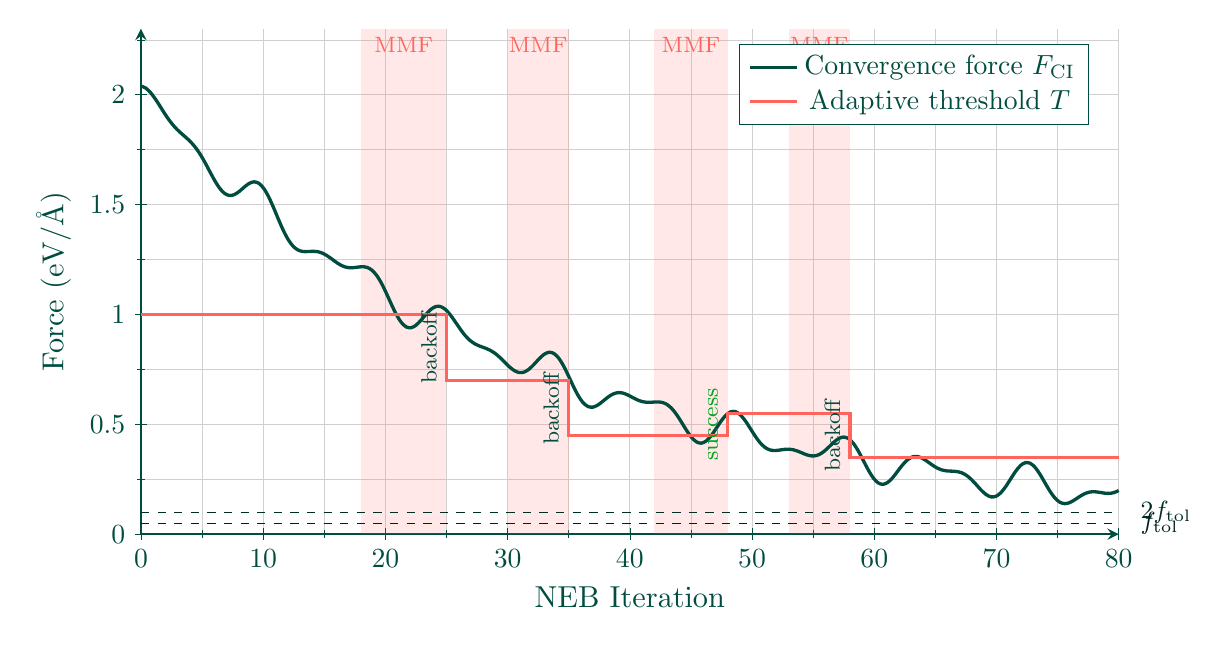
\begin{tikzpicture}
\begin{axis}[
    width=14cm,
    height=8cm,
    xmin=0, xmax=80,
    ymin=0, ymax=2.3,
    xlabel={NEB Iteration},
    ylabel={Force (eV/\AA)},
    xlabel style={font=\fontsize{11}{13}\selectfont, text=teal},
    ylabel style={font=\fontsize{11}{13}\selectfont, text=teal},
    tick label style={font=\fontsize{10}{12}\selectfont, text=teal},
    axis lines=left,
    axis line style={teal, thick},
    tick style={teal},
    minor grid style={lightgray, very thin},
    major grid style={lightgray, thin},
    grid=both,
    minor tick num=1,
    legend style={
      at={(0.97,0.97)},
      anchor=north east,
      font=\fontsize{10}{12}\selectfont,
      draw=teal,
      fill=white,
      text=teal,
    },
    clip=false,
  ]

  % Shaded trigger zones (where F < T)
  % Zone 1: around iteration 20-25
  \fill[lightcoral, opacity=0.15] (axis cs:18,0) rectangle (axis cs:25,2.3);
  \node[font=\fontsize{8}{10}\selectfont, text=coral, anchor=south]
    at (axis cs:21.5,2.15) {MMF};

  % Zone 2: around iteration 30-35
  \fill[lightcoral, opacity=0.15] (axis cs:30,0) rectangle (axis cs:35,2.3);
  \node[font=\fontsize{8}{10}\selectfont, text=coral, anchor=south]
    at (axis cs:32.5,2.15) {MMF};

  % Zone 3: around iteration 42-48
  \fill[lightcoral, opacity=0.15] (axis cs:42,0) rectangle (axis cs:48,2.3);
  \node[font=\fontsize{8}{10}\selectfont, text=coral, anchor=south]
    at (axis cs:45,2.15) {MMF};

  % Zone 4: around iteration 53-58
  \fill[lightcoral, opacity=0.15] (axis cs:53,0) rectangle (axis cs:58,2.3);
  \node[font=\fontsize{8}{10}\selectfont, text=coral, anchor=south]
    at (axis cs:55.5,2.15) {MMF};

  % Convergence force curve F_CI (smooth decreasing with slight noise)
  \addplot[teal, very thick, smooth, samples=200, domain=0:80]
    {2.0*exp(-0.03*x) + 0.06*sin(deg(x*0.8)) + 0.04*cos(deg(x*1.3))};
  \addlegendentry{Convergence force $F_{\mathrm{CI}}$}

  % Adaptive threshold T (step function)
  \addplot[coral, very thick, const plot]
    coordinates {
      (0,  1.00)
      (25, 1.00)
      (25, 0.70)
      (35, 0.70)
      (35, 0.45)
      (48, 0.45)
      (48, 0.55)
      (58, 0.55)
      (58, 0.35)
      (80, 0.35)
    };
  \addlegendentry{Adaptive threshold $T$}

  % Horizontal reference: 2*f_tol
  \addplot[teal!60!black, dashed, thin]
    coordinates {(0,0.10) (80,0.10)};
  \node[font=\fontsize{9}{11}\selectfont, text=teal!60!black, anchor=west]
    at (axis cs:81,0.10) {$2 f_{\mathrm{tol}}$};

  % Horizontal reference: f_tol
  \addplot[teal!40!black, dashed, thin]
    coordinates {(0,0.05) (80,0.05)};
  \node[font=\fontsize{9}{11}\selectfont, text=teal!40!black, anchor=west]
    at (axis cs:81,0.05) {$f_{\mathrm{tol}}$};

  % Annotations for backoff and success events
  \node[font=\fontsize{8}{10}\selectfont, text=teal, anchor=south, rotate=90]
    at (axis cs:25,0.85) {backoff};
  \node[font=\fontsize{8}{10}\selectfont, text=teal, anchor=south, rotate=90]
    at (axis cs:35,0.57) {backoff};
  \node[font=\fontsize{8}{10}\selectfont, text=teal!50!green, anchor=south, rotate=90]
    at (axis cs:48,0.50) {success};
  \node[font=\fontsize{8}{10}\selectfont, text=teal, anchor=south, rotate=90]
    at (axis cs:58,0.45) {backoff};

\end{axis}
\end{tikzpicture}
\end{document}
